%!TEX program = xelatex
%%%%%%%%%%%%%%%%%%%%%%%%%%%%%%%%%%%%%%%%%%%
%\documentclass[12pt, a4paper, fullpage]{yzu_report}
%\documentclass[12pt, a4paper, fullpage]{uiucthesis}
\documentclass[12pt, a4paper, fullpage]{mythesis}

%\usepackage{definition}
\usepackage{hyperref}
\usepackage[numbered]{bookmark}



\usepackage{cite}
\usepackage{geometry}
\usepackage{amsmath}
\usepackage{amssymb}
\usepackage{mathrsfs}
\usepackage{listings}
\usepackage{amsthm} 

\newtheorem{definition}{Definition}[section]
\newtheorem{defi}{Definition}[section]
\newtheorem{theorem}{Theorem}[section]
\newtheorem{lemma}{Lemma}[section]
%\newtheorem{proposition}{Proposition}

%\usepackage{ctex}
\usepackage{xmpmulti}
\usepackage{psfrag}
\usepackage{array}
\usepackage{graphicx}
\usepackage{caption}
\usepackage{subcaption}
\usepackage{booktabs}
\usepackage{threeparttable}
\usepackage{colortbl}
\usepackage{multirow}
\usepackage{footnote}
\usepackage{bm}
\usepackage{cases}
\usepackage{algorithm,algcompatible}
\usepackage{mathtools}
\usepackage{url}
\usepackage{rotating}


\usepackage{color}
\usepackage{rotating}
\usepackage{multicol}
\usepackage{dcolumn}
\usepackage{indentfirst}
\usepackage{makecell}
\usepackage{leftidx}
\usepackage{slashbox}
%\usepackage{subfigure}
\usepackage{fancyhdr}
% 如果不需要任何浮水印,則請把下列介於 >>> 與 <<< 之間
% 的文字行關掉 (行首加上百分號)
%% 浮水印 >>> 
% !TEX root = Thesis.tex
% this file is encoded in utf-8
% v2.0 (Apr. 5, 2009)
% 如果浮水印不是全篇需要,請把下列介於 >>> 與 <<<
% 的「全篇浮水印專用碼」關掉 (行首加百分號)
% 參考自 Keith Reckdahl 寫的 "Using Imported Graphics in LATEX2e" (epslatex.pdf) p.39
% 如果只有特定頁需要浮水印
% 則依該頁屬性使用下列之一的命令 
% 普通頁命令 \thispagestyle{WaterMarkPage}
% plain 頁命令 \thispagestyle{PlainWaterMarkPage}
% empty 頁命令 \thispagestyle{EmptyWaterMarkPage}


% 將重複使用的浮水印章
% 圖檔是 my_watermark.xxx (nctu_logo)
% 副檔名可以不加,可以是 latex 系統能處裡的任何格式:pdf, gif, png, jpg, eps, ...
% 某些圖檔格式在某些工作流程可能需要作前置處裡。
% 例如,pdflatex 無法直接處理 eps 檔
%  latex + dvipdfmx 無法直接處理 pdf, gif, png, jpg, 需要用 ebb 小工具程式
%  對圖檔產生 .bb 對應檔。
%
% 寬為 5.1 cm
\newsavebox{\mywatermark}
\sbox{\mywatermark}{
\includegraphics[keepaspectratio,width=5.1cm]{nctu_logo}}


% 將 central header 擺放浮水印的巨集指令
\newcommand{\PlaceWaterMark}{\fancyhead[C]{\setlength{\unitlength}{1in}%
\begin{picture}(0,0)%
\put(-1,-6.2){\usebox{\mywatermark}}% 圖檔擺放的位置座標
\end{picture}}%
}

%\fancyhead{}  % reset left, central, right header to empty
%% 如果不需整篇論文都要浮水印
%% 則下面  >>> 與 <<< 之間的程式碼請關閉
%% >>> 全篇浮水印

\PlaceWaterMark  % 每一頁都有浮水印 (除了 plain、empty 頁以外)

% 重新定義 plain 頁面
% 每張 plain 頁面 (每一章的第一頁) 也加浮水印

%\fancypagestyle{plain}{%
%\fancyhead{}%
%\PlaceWaterMark%
%\fancyfoot{}%
%\fancyfoot[C]{\thepage}
%\renewcommand{\headrulewidth}{0pt}%
%\renewcommand{\footrulewidth}{0pt}%
%}
%% <<< 全篇浮水印

%% 如果只有一、兩頁需要有浮水印
%% 可以在該頁 (有頁碼) 使用 \thispagestyle{WaterMarkPage}
%% 此命令不影響原有的 header、footer
%\fancypagestyle{WaterMarkPage}{%
%\PlaceWaterMark%
%}

%% 如果只有一、兩頁 plain 頁需要有浮水印 (如 摘要、自傳等)
%% 可以在該頁 (有頁碼) 使用 \thispagestyle{PlainWaterMarkPage}
%% 只有頁碼與浮水印,沒有其他的 header、footer
%% 等同於 plain page style + water mark
%\fancypagestyle{PlainWaterMarkPage}{%
%\fancyhead{}%
%\PlaceWaterMark%
%\fancyfoot{}%
%\fancyfoot[C]{\thepage}
%\renewcommand{\headrulewidth}{0pt}%
%\renewcommand{\footrulewidth}{0pt}%
%}

%% 如果只有一、兩頁 empty 頁需要有浮水印 (如封面、書名頁)
%% 可以在該頁 (無頁碼) 使用 \thispagestyle{EmptyWaterMarkPage}
%% 等同於 empty page style + water mark
\fancypagestyle{EmptyWaterMarkPage}{%
\fancyhead{}%
%\PlaceWaterMark%
\fancyfoot{}%
\renewcommand{\headrulewidth}{0pt}%
\renewcommand{\footrulewidth}{0pt}%
}
%% <<< 浮水印


\pagenumbering{arabic}

\usepackage{geometry}  % for easy margin settings
% margins setting
%\geometry{verbose,a4paper,tmargin=2.5cm,bmargin=3.5cm,lmargin=2.5cm,rmargin=2cm}



\geometry{verbose,a4paper,tmargin=2.5cm,bmargin=3.5cm,lmargin=2.5cm,rmargin=2.5cm}

\makesavenoteenv{tabular}
\renewcommand{\labelenumi}{\alph{enumi})}
%\theoremstyle{remark}
\newtheoremstyle{mythmsty}{3pt}{3pt}{}{}{\bf}{.}{.5em}{}
\theoremstyle{mythmsty}
\newtheorem{proposition}{Proposition}[chapter]
%% ENVIRONEMTS
\def\QED{\mbox{\rule[0pt]{1.5ex}{1.5ex}}}
\def\myproof{\noindent\hspace{2em}{\it Proof: }}
\def\endmyproof{\hspace*{\fill}~\QED\par\endtrivlist\unskip}
%%%%%%%%%%%%%%%%%%%%%%%%%%%%%%%%

\usepackage{type1cm}
\usepackage{fontspec}			        %加這個就可以設定字體
\usepackage{xeCJK} 			            %讓中英文字體分開設置
\XeTeXlinebreaklocale "zh"           	%這兩行一定要加,中文才能自動換行
\XeTeXlinebreakskip = 0pt plus 1pt   	%這兩行一定要加,中文才能自動換行
			                        				%加了這幾行後,就可以隨意的打中文,接下來的跟一般的LaTeX都一樣
			                        				%注意!!!一定要存成UTF-8編碼的文件。

%\setCJKmainfont[AutoFakeBold=6,AutoFakeSlant=.4]{標楷體}
								%設定中文為系統上的字型,而英文不去更動,使用原TeX字型
               	%AutoFakeBold設定粗體字要多粗
                %AutoFakeSlant設定斜體字要多斜,範圍-0.999到0.999,負值為往左斜
%\defaultCJKfontfeatures{AutoFakeBold=6,AutoFakeSlant=.4} %以後不用再設定粗斜
\setCJKmainfont[AutoFakeBold=6,AutoFakeSlant=.4]{[BiauKai.ttf]}
\defaultCJKfontfeatures{AutoFakeBold=6,AutoFakeSlant=.4}
\newCJKfontfamily\Kai{[BiauKai.ttf]}       	%定義指令\Kai則切換成標楷體
%\newCJKfontfamily\Hei{微軟正黑體}   	%定義指令\Hei則切換成正黑體
%\newCJKfontfamily\NewMing{新細明體} 	%定義指令\NewMing則切換成新細明體

\setlength{\headheight}{15pt}
%%%%%%%%%%%%%%%%%%%%%%%%%%%%%%%%
\begin{document}

%\title{Parallel Turbo Decoder Design and Implementation}  
%\author{Cheng-Chi Wong}
%\phdthesis
%\department{Department of Electronics Engineering \& Institute of Electronics}
%\college{Electrical \& Computer Engineering} 
%\advisor{Hsie-Chia Chang}
%\degreeyear{2010}

%\maketitle

\frontmatter

% !TEX root = Thesis.tex
%
% this file is encoded in utf-8
% v2.0 (Apr. 5, 2009)

% ??????????????????????
% ??????????? (??) ??
% ?? \prechaptername ???? Chapter
% ?? \postchaptername ???????
% ?? \tablename ???? Table
% ?? \figurename ???? Figure
%\renewcommand\prechaptername{?} % ???????????? x ??
%\renewcommand\postchaptername{?}
%\renewcommand{\tablename}{?} % ???? table caption ???? x???
%\renewcommand{\figurename}{?} % ???? figure caption ???? x???

% ??????????????????????? (??????????)
%\newcommand{\nameInnerCover}{???}
%\newcommand{\nameCommitteeForm}{?????????}
%\newcommand{\nameCopyrightForm}{???}
%\newcommand{\nameCabstract}{????}
%\newcommand{\nameEabstract}{????}
%\newcommand{\nameAckn}{??}
%\newcommand{\nameToc}{??}
%\newcommand{\nameLot}{???}
%\newcommand{\nameTof}{???}
%\newcommand{\nameSlist}%{????}
\newcommand{\nameSlist}{Symbol List}
%\newcommand{\nameRef}{????}
%\newcommand{\nameVita}{??}


%!TEX root = Thesis.tex
%
% this file is encoded in utf-8
% v2.0 (Apr. 5, 2009)
% do not change the content of this file
% unless the thesis layout rule is changed
% 無須修改本檔內容,除非校方修改了
% 封面、書名頁、中文摘要、英文摘要、誌謝、目錄、表目錄、圖目錄、符號說明
% 等頁之格式


% default variables definitions
% 此處只是預設值,不需更改此處
% 請更改 my_names.tex 內容
\newcommand\cTitle{論文題目}
\newcommand\eTitle{MY THESIS TITLE}
\newcommand\myCname{我的中文名字}
\newcommand\myEname{My Name}
\newcommand\advisorCnameA{第一指導教授中文名字}
\newcommand\advisorEnameA{Name of the 1st Advisor}
\newcommand\advisorCnameB{第二指導教授中文名字}
\newcommand\advisorEnameB{Name of the 2nd Advisor}
\newcommand\advisorCnameC{第三指導教授中文名字}
\newcommand\advisorEnameC{Name of the 3rd Advisor}
\newcommand\univCname{大學名稱}
\newcommand\univEname{University}
\newcommand\deptCname{系所名稱}
\newcommand\fulldeptEname{Department}
\newcommand\deptEname{Department}
\newcommand\collEname{College}
\newcommand\degreeCname{學位}
\newcommand\degreeEname{Degree}
\newcommand\cYear{民國年份}
\newcommand\cMonth{月數}
\newcommand\eYear{Year}
\newcommand\eMonth{Month}
\newcommand\ePlace{Location of University}

% user's names; to replace those default variable definitions
% this file is encoded in utf-8
% v2.0 (Apr. 5, 2009)
% 填入你的論文題目、姓名等資料
% 如果題目內有必須以數學模式表示的符號,請用 \mbox{} 包住數學模式,如下範例
% 如果中文名字是單名,與姓氏之間建議以全形空白填入,如下範例
% 英文名字中的稱謂,如 Prof. 以及 Dr.,其句點之後請以不斷行空白~代替一般空白,如下範例
% 如果你的指導教授沒有如預設的三位這麼多,則請把相對應的多餘教授的中文、英文名
%    的定義以空的大括號表示
%    如,\renewcommand\advisorCnameB{}
%          \renewcommand\advisorEnameB{}
%          \renewcommand\advisorCnameC{}
%          \renewcommand\advisorEnameC{}

% 論文題目 (中文)
\renewcommand\cTitle{類比電路自動化與遷移設計之研究}

% 論文題目 (英文)
\renewcommand\eTitle{Research on Analog Design Automation and Migration}

% 我的姓名 (中文)
\renewcommand\myCname{潘柏丞}

% 我的姓名 (英文)
\renewcommand\myEname{Po-Cheng Pan}

% 指導教授A的姓名 (中文)
\renewcommand\advisorCnameA{陳宏明}

% 指導教授A的姓名 (英文)
\renewcommand\advisorEnameA{Hung-Ming Chen}

% 指導教授B的姓名 (中文)
\renewcommand\advisorCnameB{}

% 指導教授B的姓名 (英文)
\renewcommand\advisorEnameB{}

% 指導教授C的姓名 (中文)
\renewcommand\advisorCnameC{}

% 指導教授C的姓名 (英文)
\renewcommand\advisorEnameC{}

% 校名 (中文)
\renewcommand\univCname{國立交通大學}

% 校名 (英文)
\renewcommand\univEname{National Chiao Tung University}

% 系所名 (中文)
\renewcommand\deptCname{電子工程學系電子研究所}

% 系所全名 (英文)
\renewcommand\fulldeptEname{Department of Electronics Engineering \& Institute of Electronics}

% 系所短名 (英文, 用於書名頁學位名領域)
\renewcommand\deptEname{Electronics Engineering}

% 學院英文名 (如無,則以空的大括號表示)
\renewcommand\collEname{College of Electrical and Computer Engineering}

% 學位名 (中文)
\renewcommand\degreeCname{博士}

% 學位名 (英文)
\renewcommand\degreeEname{Doctor of Philosophy}

% 口試年份 (中文、民國)
\renewcommand\cYear{一零四}

% 口試月份 (中文)
\renewcommand\cMonth{五} 

% 口試年份 (阿拉伯數字、西元)
\renewcommand\eYear{2015} 

% 口試月份 (英文)
\renewcommand\eMonth{May}

% 學校所在地 (英文)
\renewcommand\ePlace{Hsinchu, Taiwan, Republic of China}

%畢業級別;用於書背列印;若無此需要可忽略
\newcommand\GraduationClass{103}

%%%%%%%%%%%%%%%%%%%%%%


% make the line spacing in effect
%\newcommand{\mybaselinestretch}{1.5}  %行距 1.5 倍 + 20%, (約為 double space)
%\renewcommand{\baselinestretch}{\mybaselinestretch}  % 論文行距預設值
%\parskip = 2ex                                       % 段落之間的間隔為兩個 x 的高度
%\parindent = 0Pt                                     % 這裡設成不內縮

%\renewcommand{\baselinestretch}{\mybaselinestretch}
\large % it needs a font size changing command to be effective

\newcommand\itsempty{}
%%%%%%%%%%%%%%%%%%%%%%%%%%%%%%%
%        cover 封面
%%%%%%%%%%%%%%%%%%%%%%%%%%%%%%%

\begin{titlepage}
% no page number
% next page will be page 1

\ifx\mywatermark\undefined 
  \thispagestyle{empty}  % 無頁碼、無 header (無浮水印)
\else
  \thispagestyle{EmptyWaterMarkPage} % 無頁碼、有浮水印
\fi

% aligned to the center of the page
\begin{center}
% font size (relative to 12 pt):
% \large (14pt) < \Large (18pt) < \LARGE (20pt) < \huge (24pt)< \Huge (24 pt)
%
%\makebox[12cm][s]{\Huge{\univCname}}\\  %顯示中文校名
\makebox[12cm][s]{\fontsize{36pt}{10pt}\selectfont{\univCname}}\\
\vspace{1.5cm}
%\makebox[12cm][s]{\huge{\deptCname}}\\ %顯示中文系所名
\makebox[12cm][s]{\fontsize{28pt}{10pt}\selectfont{\deptCname}}\\
\vspace{1.5cm}
%\makebox[6cm][s]{\huge{\degreeCname 論文}}\\ %顯示論文種類 (中文)
\makebox[6cm][s]{\fontsize{28pt}{10pt}\selectfont{\degreeCname 論文}}\\
\vspace{2cm}
%
% Set the line spacing to single for the titles (to compress the lines)
%\renewcommand{\baselinestretch}{1}   %行距 1 倍
\large % it needs a font size changing command to be effective
\LARGE{\cTitle}\\  % 中文題目
%
%\vspace{1cm}
%
\LARGE{\eTitle}\\ %英文題目
\vspace{2cm}
% \makebox is a text box with specified width;
% option s: stretch
% use \makebox to make sure
% 「研究生:」 與「指導教授:」occupy the same width
\hspace{4.5cm} \makebox[4cm][s]{\LARGE{研究生}} \makebox[0.5cm][c]{\LARGE{:}}
\LARGE{\myCname}  % 顯示作者中文名
\hfill \makebox[1cm][s]{}\\
%
\hspace{4.5cm} \makebox[4cm][s]{\LARGE{指導教授}}  \makebox[0.5cm][c]{\LARGE{:}}
\LARGE{\advisorCnameA}  %顯示指導教授A中文名
\hfill \makebox[1cm][s]{}\\
%
% 判斷是否有共同指導的教授 B
\ifx \advisorCnameB  \itsempty
\relax % 沒有 B 教授,所以不佔版面,不印任何空白
\else
% 共同指導的教授 B
\hspace{4.5cm} \makebox[4cm][s]{} \makebox[0.5cm][c]{}
\LARGE{\advisorCnameB}  %顯示指導教授B中文名
\hfill \makebox[1cm][s]{}\\
\fi
%
% 判斷是否有共同指導的教授 C
\ifx \advisorCnameC  \itsempty
\relax % 沒有 C 教授,所以不佔版面,不印任何空白
\else
% 共同指導的教授 C
\hspace{4.5cm} \makebox[3cm][s]{}
\LARGE{\advisorCnameC}  %顯示指導教授C中文名
\hfill \makebox[1cm][s]{}\\
\fi
%
\vfill
\makebox[10cm][s]{\LARGE{中華民國\cYear 年\cMonth 月}}%
%
\end{center}
% Resume the line spacing to the desired setting
%\renewcommand{\baselinestretch}{\mybaselinestretch}   %恢復原設定
% it needs a font size changing command to be effective
% restore the font size to normal
\normalsize
\end{titlepage}
%%%%%%%%%%%%%%

%% 從摘要到本文之前的部份以小寫羅馬數字印頁碼
% 但是從「書名頁」(但不印頁碼) 就開始計算
\setcounter{page}{1}
\pagenumbering{roman}
%%%%%%%%%%%%%%%%%%%%%%%%%%%%%%%
%       書名頁 
%%%%%%%%%%%%%%%%%%%%%%%%%%%%%%%
\newpage

% 判斷是否要浮水印?
\ifx\mywatermark\undefined 
  \thispagestyle{empty}  % 無頁碼、無 header (無浮水印)
\else
  \thispagestyle{EmptyWaterMarkPage} % 無頁碼、有浮水印
\fi

%no page number
% create an entry in table of contents for 書名頁
%%\phantomsection % for hyperref to register this
%%\addcontentsline{toc}{chapter}{\nameInnerCover}


% aligned to the center of the page
\begin{center}
% font size (relative to 12 pt):
% \large (14pt) < \Large (18pt) < \LARGE (20pt) < \huge (24pt)< \Huge (24 pt)
% Set the line spacing to single for the titles (to compress the lines)
%%\renewcommand{\baselinestretch}{1}   %行距 1 倍
% it needs a font size changing command to be effective
%中文題目
\Large{\cTitle}\\ %%%%%
%\vspace{1cm}
% 英文題目
\Large{\eTitle}\\ %%%%%
%\vspace{1cm}
\vfill
% \makebox is a text box with specified width;
% option s: stretch
% use \makebox to make sure
% 「研究生:」 與「指導教授:」occupy the same width
\makebox[3cm][s]{\large{研 究 生}} \makebox{\large{:}}
\makebox[3cm][l]{\large{\myCname}} %%%%%
\hfill
\makebox[1.5cm][s]{\large{Student}} \makebox{\large{:}}
\makebox[5cm][l]{\large{\myEname}}\\ %%%%%
%
%\vspace{1cm}
%
\makebox[3cm][s]{\large{指導教授}} \makebox{\large{:}}
\makebox[4cm][l]{\large{\advisorCnameA} \large{博士}} %%%%%
%\makebox[1cm][l]{\large{博士}}
\hfill
\makebox[1.5cm][s]{\large{Advisor}} \makebox{\large{:}}
\makebox[5cm][l]{\large{Dr. \advisorEnameA}}\\ %%%%%
%
% 判斷是否有共同指導的教授 B
\ifx \advisorCnameB  \itsempty
\relax % 沒有 B 教授,所以不佔版面,不印任何空白
\else
%共同指導的教授B
\makebox[3cm][s]{}
%\makebox[3cm][l]{\large{\advisorCnameB}} %%%%%
\makebox[0.5cm][l]{}
\makebox[4cm][l]{\large{\advisorCnameB} \large{博士}} %%%%%
\hfill
\makebox[2cm][s]{}
\makebox[5cm][l]{\large{Dr. \advisorEnameB}}\\ %%%%%%%%%%%%%%%%%%%%%%%%%%%%%%%%%%%%%%%%%%%%%%%%%%%%%%%%%%%%%%%%%%%%%%%%%%%%%%%%%%%%%%%%%%%%%%%%%%%%%%%%%%%%%%%%%%%%%
\fi
%
% 判斷是否有共同指導的教授 C
\ifx \advisorCnameC  \itsempty
\relax % 沒有 C 教授,所以不佔版面,不印任何空白
\else
%共同指導的教授C
\makebox[3cm][s]{}
\makebox[3cm][l]{\large{\advisorCnameC}} %%%%%
\hfill
\makebox[2cm][s]{}
\makebox[5cm][l]{\large{\advisorEnameC}}\\ %%%%%
\fi
%
% Resume the line spacing to the desired setting
%\renewcommand{\baselinestretch}{\mybaselinestretch}   %恢復原設定
\large %it needs a font size changing command to be effective
%
\vfill
\makebox[4cm][s]{\large{\univCname}}\\% 校名
\makebox[6cm][s]{\large{\deptCname}}\\% 系所名
\makebox[3cm][s]{\large{\degreeCname 論文}}\\% 學位名
%
%\vspace{1cm}
\vfill
%%\large{A Dissertation}\\%
\normalsize{A Dissertation}\\
%%\large{Submitted to}%
\normalsize{Submitted to}
%
%%\large{\fulldeptEname}\\%系所全名 (英文)
\normalsize{\fulldeptEname}\\
%
%
\ifx \collEname  \itsempty
\relax % 沒有學院名 (英文),所以不佔版面,不印任何空白
\else
% 有學院名 (英文)
%%\large{\collEname}\\% 學院名 (英文)
\normalsize{\collEname}\\
\fi
%
%%\large{\univEname}\\%校名 (英文)
\normalsize{\univEname}\\
%
%%\large{in Partial Fulfillment of the Requirements}\\
\normalsize{in Partial Fulfillment of the Requirements}\\
%
%%\large{for the Degree of}
\normalsize{for the Degree of}
%
%%\large{\degreeEname}\\%學位名(英文)
\normalsize{\degreeEname}\\
%
%%\large{in}\\
\normalsize{in}\\
%
%%\large{\deptEname}\\%系所短名(英文;表明學位領域)
\normalsize{\deptEname}\\
%
%%\large{\eMonth\ \eYear}\\%月、年 (英文)
\normalsize{\eMonth\ \eYear}\\
%
%%\large{\ePlace}% 學校所在地 (英文)
\normalsize{\ePlace}% 學校所在地 (英文)
\vfill
\large{中華民國}%
\large{\cYear}% %%%%%
\large{年}%
\large{\cMonth}% %%%%%
\large{月}\\
\end{center}
% restore the font size to normal
\normalsize
\clearpage


%%%%%%%%%%%%%%%%%%%%%%%%%%%%%%%
%       論文口試委員審定書 (計頁碼,但不印頁碼) 
%%%%%%%%%%%%%%%%%%%%%%%%%%%%%%%


%%%%%%%%%%%%%%%%%%%%%%%%%%%%%%%
%       授權書 (計頁碼,但不印頁碼) 
%%%%%%%%%%%%%%%%%%%%%%%%%%%%%%%

























%%%%%%%%%%%%%%%%%%%%%%%%%%%%%%%%
%%       中文摘要 
%%%%%%%%%%%%%%%%%%%%%%%%%%%%%%%%
%
\newpage
\thispagestyle{plain}  % 無 header,但在浮水印模式下會有浮水印

% create an entry in table of contents for 中文摘要
%%\phantomsection % for hyperref to register this
%%\addcontentsline{toc}{chapter}{\nameCabstract}

% aligned to the center of the page
\begin{center}
% font size (relative to 12 pt):
% \large (14pt) < \Large (18pt) < \LARGE (20pt) < \huge (24pt)< \Huge (24 pt)
% Set the line spacing to single for the names (to compress the lines)
%%\renewcommand{\baselinestretch}{1}   %行距 1 倍
% it needs a font size changing command to be effective
\Large{\cTitle}\\  %中文題目
\vspace{0.83cm}
% \makebox is a text box with specified width;
% option s: stretch
% use \makebox to make sure
% each text field occupies the same width
\makebox[1.5cm][s]{\large{學生:}}
\makebox[3cm][l]{\large{\myCname}} %學生中文姓名
\hfill
%
\makebox[3cm][s]{\large{指導教授:}}
\makebox[3cm][l]{\large{\advisorCnameA}\large{教授}} \\ %教授A中文姓名
%
% 判斷是否有共同指導的教授 B
\ifx \advisorCnameB  \itsempty
\relax % 沒有 B 教授,所以不佔版面,不印任何空白
\else
%共同指導的教授B
\makebox[1.5cm][s]{}
\makebox[3cm][l]{} %%%%%
\hfill
\makebox[3cm][s]{}
\makebox[3cm][l]{\large{\advisorCnameB}\large{教授}}\\ %教授B中文姓名
\fi
%
% 判斷是否有共同指導的教授 C
\ifx \advisorCnameC  \itsempty
\relax % 沒有 C 教授,所以不佔版面,不印任何空白
\else
%共同指導的教授C
\makebox[1.5cm][s]{}
\makebox[3cm][l]{} %%%%%
\hfill
\makebox[3cm][s]{}
\makebox[3cm][l]{\large{\advisorCnameC}\large{教授}}\\ %教授C中文姓名
\fi
%
\vspace{0.42cm}
%
\large{\univCname}\large{\deptCname}\\ %校名系所名
\vspace{0.83cm}
%\vfill
\makebox[2.5cm][s]{\large{摘要}}\\
\end{center}
% Resume the line spacing to the desired setting
%%\renewcommand{\baselinestretch}{\mybaselinestretch}   %恢復原設定
%it needs a font size changing command to be effective
% restore the font size to normal
\normalsize
%%%%%%%%%%%%%
% !TEX root = Thesis.tex

在積體電路的範疇,為了更有效地達到先進製程底下的電路效能,類比電路的自動化已不容忽視。以下自行發揮

























%%%%%%%%%%%%%%%%%%%%%%%%%%%%%%%
%       英文摘要 
%%%%%%%%%%%%%%%%%%%%%%%%%%%%%%%
%
\newpage
\thispagestyle{plain}  % 無 header,但在浮水印模式下會有浮水印

% create an entry in table of contents for 英文摘要
%%\phantomsection % for hyperref to register this
%%\addcontentsline{toc}{chapter}{\nameEabstract}

% aligned to the center of the page
\begin{center}
% font size:
% \large (14pt) < \Large (18pt) < \LARGE (20pt) < \huge (24pt)< \Huge (24 pt)
% Set the line spacing to single for the names (to compress the lines)
%%\renewcommand{\baselinestretch}{1}   %行距 1 倍
%\large % it needs a font size changing command to be effective
\Large{\eTitle}\\  %英文題目
\vspace{0.83cm}
% \makebox is a text box with specified width;
% option s: stretch
% use \makebox to make sure
% each text field occupies the same width
\makebox[2cm][s]{\large{Student: }}
\makebox[5cm][l]{\large{\myEname}} %學生英文姓名
\hfill
%
\makebox[2cm][s]{\large{Advisor: }}
\makebox[5cm][l]{\large{\advisorEnameA}} \\ %教授A英文姓名
%
% 判斷是否有共同指導的教授 B
\ifx \advisorCnameB  \itsempty
\relax % 沒有 B 教授,所以不佔版面,不印任何空白
\else
%共同指導的教授B
\makebox[2cm][s]{}
\makebox[5cm][l]{} %%%%%
\hfill
\makebox[2cm][s]{}
\makebox[5cm][l]{\large{\advisorEnameB}}\\ %教授B英文姓名
\fi
%
% 判斷是否有共同指導的教授 C
\ifx \advisorCnameC  \itsempty
\relax % 沒有 C 教授,所以不佔版面,不印任何空白
\else
%共同指導的教授C
\makebox[2cm][s]{}
\makebox[5cm][l]{} %%%%%
\hfill
\makebox[2cm][s]{}
\makebox[5cm][l]{\large{\advisorEnameC}}\\ %教授C英文姓名
\fi
%
\vspace{0.42cm}
%%\large{Submitted to }\large{\fulldeptEname}\\  %英文系所全名
\large{\fulldeptEname}\\  %英文系所全名
%
%  建議不用加學院名稱
\ifx \collEname  \itsempty
\relax % 如果沒有學院名 (英文),則不佔版面,不印任何空白
\else
% 有學院名 (英文)
\large{\collEname}\\% 學院名 (英文)
\fi
%
\large{\univEname}\\  %英文校名
\vspace{0.83cm}
%\vfill
%
\large{ABSTRACT}\\
%\vspace{0.5cm}
\end{center}
% Resume the line spacing the desired setting
%%\renewcommand{\baselinestretch}{\mybaselinestretch}   %恢復原設定
%\large %it needs a font size changing command to be effective
% restore the font size to normal
\normalsize
%%%%%%%%%%%%%
% !TEX root = Thesis.tex

This dissertation presents an analog automation flow and design migration methodology
%both nonuniversal and universal approaches that improve the performance of short-length Luby Transform (LT) codes with applications to multimedia communication. The key idea is to increase the expected \emph{output ripple size} to prevent Belief-Propagation (BP) decoding process from terminating prematurely. The nonuniversal approach with Soliton-based distribution and randomness-limited encoding scheme is discussed first. Then the universal approach is investigated focusing on constructing degree distributions with respect to the output ripple size.


%, where the output ripple size is the number of degree-$1$ output symbols


%LT codes have been proved to be capacity-achieving on erasure channels. The performance of these codes is dominated by the code length and the design of the degree distribution. The state of the art robust Soliton distribution (RSD) is designed for asymptotic optimality and widely used in communication systems. As the code length decreases, however, the performance of LT codes using RSD degrades. This is because the output ripple size becomes smaller and more likely to decrease to zero during early stage, leading to frequent premature decoding termination. As a result, RSD is unsuitable for multimedia communication, which typically involves transmission of small or segmented data, such as music files and Group of Pictures (GOP) in a coded video.


% since its expected output ripple size is relatively small during early decoding stage where decoding terminations 


%In the nonuniversal approach, we increase the degree-$1$ proportion in RSD. The output ripple size becomes larger accordingly, and the problem of premature decoding termination is then relieved. The proportion of low degrees, except for degree-$1$, is also decreased to reduce the number of redundant output symbols. In addition, we introduce \emph{Non-Repetitive} (NR) encoding scheme to avoid generating repeated degree-$1$ output symbols. NR encoding scheme limits the randomness of the encoding process so that its performance depends on the channel condition. Moreover, we integrate multiple NR encoders to achieve Unequal Erasure Protection (UEP) for Scalable Video Coding (SVC) layers with different importance. Experimental results show that our UEP scheme outperforms previous studies in terms of the Peak Signal-to-Noise Ratio (PSNR).



%In the universal approach, RSD is replaced by our proposed distributions. Meanwhile, we keep the encoding process intact to maintain the universality of LT codes. By minimizing objective functions under certain constraints, degree distributions can be constructed with their expected output ripple size approximating predetermined curves. Sequential Quadratic Programming (SQP) algorithm is employed to solve the minimization problem. Compared to RSD and previous works, our proposed ripple-based distribution (RBD) is able to reduce the average overhead needed to fully decode input symbols as well as the encoding and decoding complexity. Moreover, we record User Datagram Protocol (UDP) packet loss patterns over 802.11g WLAN and apply them to our simulations. The corresponding results show that the transmission efficiency can be improved by using RBD instead of RSD. Compared to RSD, RBD reduces the encoding and decoding complexity by at least $31.2\%$ and $25.4\%$, respectively.

%%%%%%%%%%%%%%%%%%%%%%%%%%%%%%%
%       誌謝 
%%%%%%%%%%%%%%%%%%%%%%%%%%%%%%%
%
% Acknowledgement
\newpage
\thispagestyle{plain}
%\chapter*{\protect\makebox[5cm][s]{\nameAckn}} %\makebox{} is fragile; need protect
%\phantomsection % for hyperref to register this
%\addcontentsline{toc}{chapter}{\nameAckn}
\begin{center}
\makebox[5cm][s]{\Large{\textbf{誌謝}}}
\end{center}
\vspace{2cm}
在漫長的五年博士班的修業過程中,如今下筆要寫出這段誌謝誠然百感交集
%承蒙師長的教誨、家人的支持以及夥伴們的合作,最終我才能完成學業。
%特別感謝張錫嘉老師的指導與提供的資源,並給予我嘗試錯誤的機會,能夠在這樣自由的環境中從事研究,我感到十分的幸福。
%同時感謝邵家健教授,讓我在修業過程中學習到寶貴的研究方法和態度。
%此外,由衷感激廖彥欽學姊、陳志龍學長及翁政吉學長,因為有你們的幫助,才能加快我研究的腳步。
%也感謝OASIS實驗室及OCEAN和邵家健教授團隊的所有成員,透過日常的討論,解答我許多課業上的疑問。
%最後要感謝我家人全心全意的支持,我才能堅定的達成每個目標。





%%%%%%%%%%%%%%%%%%%%%%%%%%%%%%%
%       目錄 
%%%%%%%%%%%%%%%%%%%%%%%%%%%%%%%
%
% Table of contents
%\newpage
\renewcommand{\contentsname}{Contents}                                                                 
%\renewcommand{\contentsname}{\protect\makebox[5cm][s]{\nameToc}}
%%\makebox{} is fragile; need protect
%\phantomsection % for hyperref to register this
%\addcontentsline{toc}{chapter}{\nameToc}
%\addcontentsline{toc}{chapter}{\contentsname}
\tableofcontents

%%%%%%%%%%%%%%%%%%%%%%%%%%%%%%%
%       表目錄 
%%%%%%%%%%%%%%%%%%%%%%%%%%%%%%%
%
% List of Tables
%\newpage
%\renewcommand{\listtablename}{\protect\makebox[5cm][s]{\nameLot}}
%%\makebox{} is fragile; need protect
%\phantomsection % for hyperref to register this
%\addcontentsline{toc}{chapter}{\nameLot}
%\addcontentsline{toc}{chapter}{\listtablename}
\listoftables

%%%%%%%%%%%%%%%%%%%%%%%%%%%%%%%
%       圖目錄 
%%%%%%%%%%%%%%%%%%%%%%%%%%%%%%%
%
% List of Figures
%\newpage
%\renewcommand{\listfigurename}{\protect\makebox[5cm][s]{\nameTof}}
%%\makebox{} is fragile; need protect
%\phantomsection % for hyperref to register this
%\addcontentsline{toc}{chapter}{\nameTof}
%\addcontentsline{toc}{chapter}{\listfigurename}
\listoffigures

%%%%%%%%%%%%%%%%%%%%%%%%%%%%%%%
%       符號說明 
%%%%%%%%%%%%%%%%%%%%%%%%%%%%%%%
%
% Symbol list
% define new environment, based on standard description environment
% adapted from p.60~64, <<The LaTeX Companion>>, 1994, ISBN 0-201-54199-8
\newcommand{\SymEntryLabel}[1]%
  {\makebox[3cm][l]{#1}}
%
\newenvironment{SymEntry}
   {\begin{list}{}%
       {\renewcommand{\makelabel}{\SymEntryLabel}%
        \setlength{\labelwidth}{3cm}%
        \setlength{\leftmargin}{\labelwidth}%
        }%
   }%
   {\end{list}}
%%
\newpage
\chapter*{\protect\makebox[5cm][s]{\nameSlist}} %\makebox{} is fragile; need protect
%\addcontentsline{toc}{chapter}{\nameSlist}
\begin{SymEntry}

\item[ARQ]
Automatic Repeat reQuest

%\item[BEC]
%Binary Erasure Channel
%\item[BL]
%Base Layer
%\item[BP]
%Belief-Propagation
%
%\item[DS]
%Duplicate-Symbols
%
%\item[EL]
%Enhancement Layer
%
%\item[FEC]
%Forward Error/Erasure Correction
%
%\item[GOP]
%Group of Pictures
%
%\item[IDR]
%Instantaneous Decoder Refresh
%\item[ISD]
%Ideal Soliton Distribution
%
%\item[KKT]
%Karush-Kuhn-Tucker
%
%\item[LDPC]
%Low-Density Parity-Check
%\item[LIB]
%Least Important Bits
%\item[LT]
%Luby Transform
%
%
%\item[MDS]
%Maximum Distance Separable
%\item[MIB]
%Most Important Bits
%\item[MRSD]
%Modified Robust Soliton Distribution
%
%\item[NALU]
%Network Abstraction Layer Units
%\item[NR]
%Non-Repetitive
%
%
%\item[PSNR]
%Peak Signal-to-Noise Ratio
%
%\item[RBD]
%Ripple-Based Distribution
%\item[RS]
%Reed-Solomon
%\item[RSD]
%Robust Soliton Distribution
% 
%
%
%\item[SQP]
%Sequential Quadratic Programming
%\item[SVC]
%Scalable Video Coding
%\item[SW]
%Sliding-Window
%
%
%\item[UDP]
%User Datagram Protocol
%\item[UEP]
%Unequal Erasure Protection
%
%
%
%
%\item[$k$]
%Code length
%
%\item[$K$]
%Number of received output symbols
%
%\item[$\epsilon$]
%Overhead ($\epsilon=\frac{K-k}{k}$)
%
%\item[$\rho$]
%Number of decoded input symbols during BP decoding process
%
%\item[$\rho/k$]
%Ratio of decoded input symbols during BP decoding process
%
%\item[$\Omega^r(x)$]
%Robust Soliton distribution (RSD)
%
%\item[$\Omega^P(x)$]
%Ripple-Based Distribution (RBD)
%
%
%\item[$\Gamma(\rho)$]
%Occurrence probability of BP decoding termination when $\rho$ input %symbols are decoded
%
%\item[$\Pi(\rho)$]
%Cumulative probability of decoding termination ($\Pi(\rho)=\sum_{q=0}^{\%rho}{\Gamma(q)}$)
%
%\item[$P_e$]
%Channel erasure rate
%
%\item[$\overline{\Delta}$]
%Average number of symbol operations to generate an encoding symbol. (A %symbol operation is either an exclusive-or between two symbols or a copy %of one symbol to another.)
%
%\item[$\overline{s}$]
%Average number of symbol operations needed to decode an input symbol
%
%\item[$\overline{m}$]
%Average number of output symbols transmitted for decoding $k$ input %symbols
%
%\item[$d(c_l)$]
%Degree of output symbol $c_l$
%
%\item[$C_r$]
%A set of $K$ received output symbols
%
%\item[$S$]
%Successful decoding probability (Probability of decoding all $k$ input %symbols from $(1+\epsilon)k$ received encoding symbols, where $S=\Gamma(%k)=1-\sum_{q=0}^{k-1}{\Gamma(q)}=1-\Pi(k-1)$)
%
%\item[$L$]
%Symbol loss probability. (Probability that an input symbol remains undecoded after BP decoding process, where $L=\sum_{\rho=0}^{k}{\frac{k-\rho}{k}\Gamma(\rho)}$.)



%$\Lambda(c_l)$ &: A set of input symbols connected by encoding symbol $c_l$ (neighbors of encoding symbol $c_l$). \\
%$\Lambda(i_l)$ &: A set of encoding symbols connecting to input symbol $i_l$ (neighbors of input symbol $i_l$). \\
%$R(\rho)$ &: Average number of degree-$1$ encoding symbols during BP decoding process when $\rho$ input symbols are decoded. \\


\end{SymEntry}


\newpage
%%% 論文本體頁碼回復為阿拉伯數字計頁,並從頭起算
\pagenumbering{arabic}
%%%%%%%%%%%%%%%%%%%%%%%%%%%%%%%%

\mainmatter
% !TEX root = Thesis.tex
\chapter{Introduction}\label{sec:Intro}

  In the late nanoscale CMOS era, automated layout generation of advanced technologies has drawn more attention due to the growing demand in industry. As the complexity of the advanced nodes for analog circuit increases, the layout constraints and the expanding performance requirements become major productivity bottlenecks. Lately, in order to alleviate the impact from process variation beyond the transistor level as well as striving for excellent performance, analog layout design mostly relies on designers' expertise. However, the iterative refinement on manual design damages the productivity of analog layout. Therefore, it is more efficient to enroll the know-how from existing designs instead of generating a new one. To migrate layout template via preservation becomes a plus.

  For analog layout, reusability relies on the similarity such that part of source layout can be reused to add new modules or layers on target layout with minor modification. To preserve the design knowledge from the template layouts, the devices' relative positions and the routing behaviors should be considered thoroughly. Typical analog constraints such as symmetry and proximity constraints fundamentally regulate the placement. On the other hand, wire symmetry and topological matching are critical to analog routing. Placement and routing extracted from the template layout can benefit layout migration. In other words, more informations are extracted from template layout, more circuit characteristics are preserved. Currently, analog layout preservation pays more attention on placement~\cite{cart-hammouda-dac06,cbc-bhattacharya-dac04,Wang_ALRGP_TODAES2011} 
  for topology extraction. However, seldom do we study routing behavior extraction in previous works. In all, a solution to preserve the correlation during layout retargeting, or so-called layout migration is critical.


  \begin{figure}
    \centering
    \begin{subfigure}[t]{4cm}
    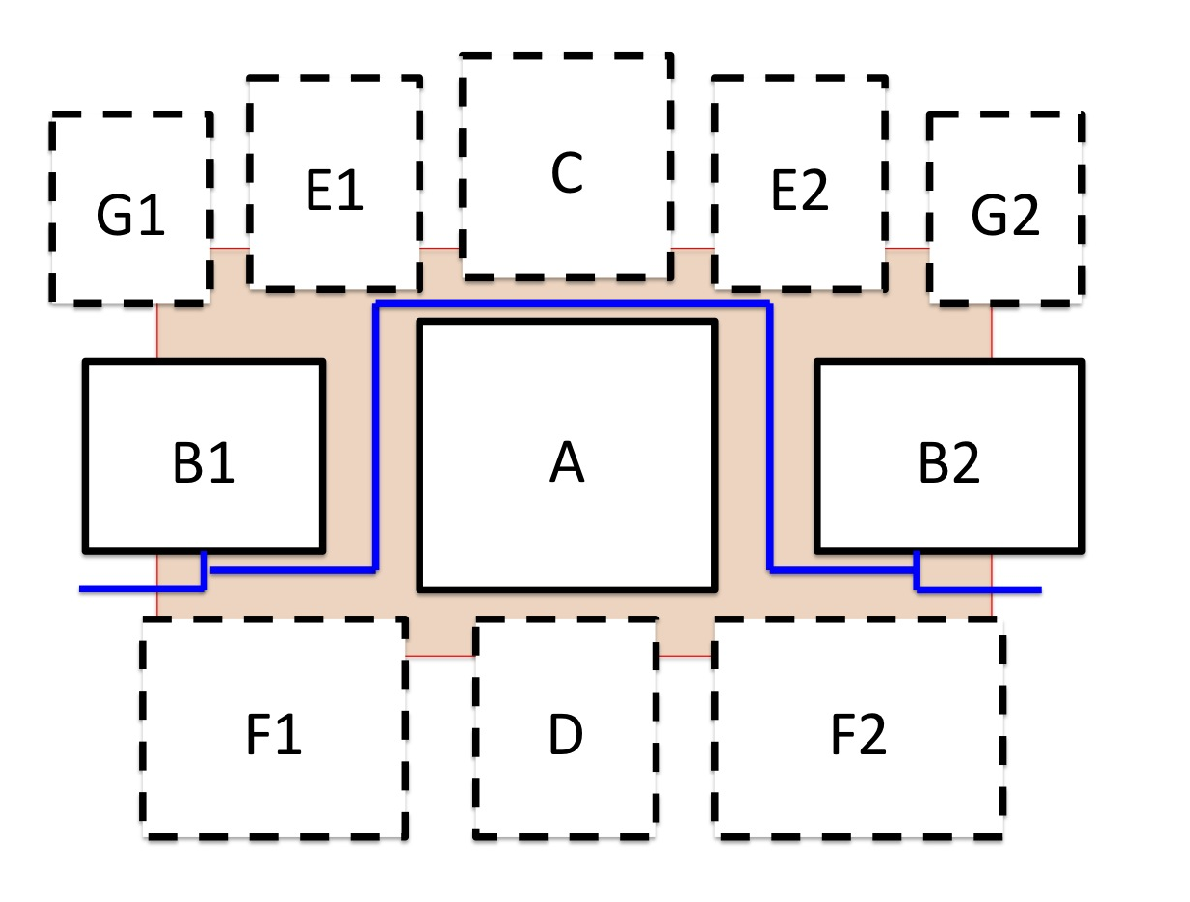
\includegraphics[width=4cm]{Fig/RoutingPreserv_a.eps}
    \caption{Reference template layout}
    \label{fig:RoutingPreserv_A}
    \end{subfigure}
    \begin{subfigure}[t]{4cm}
    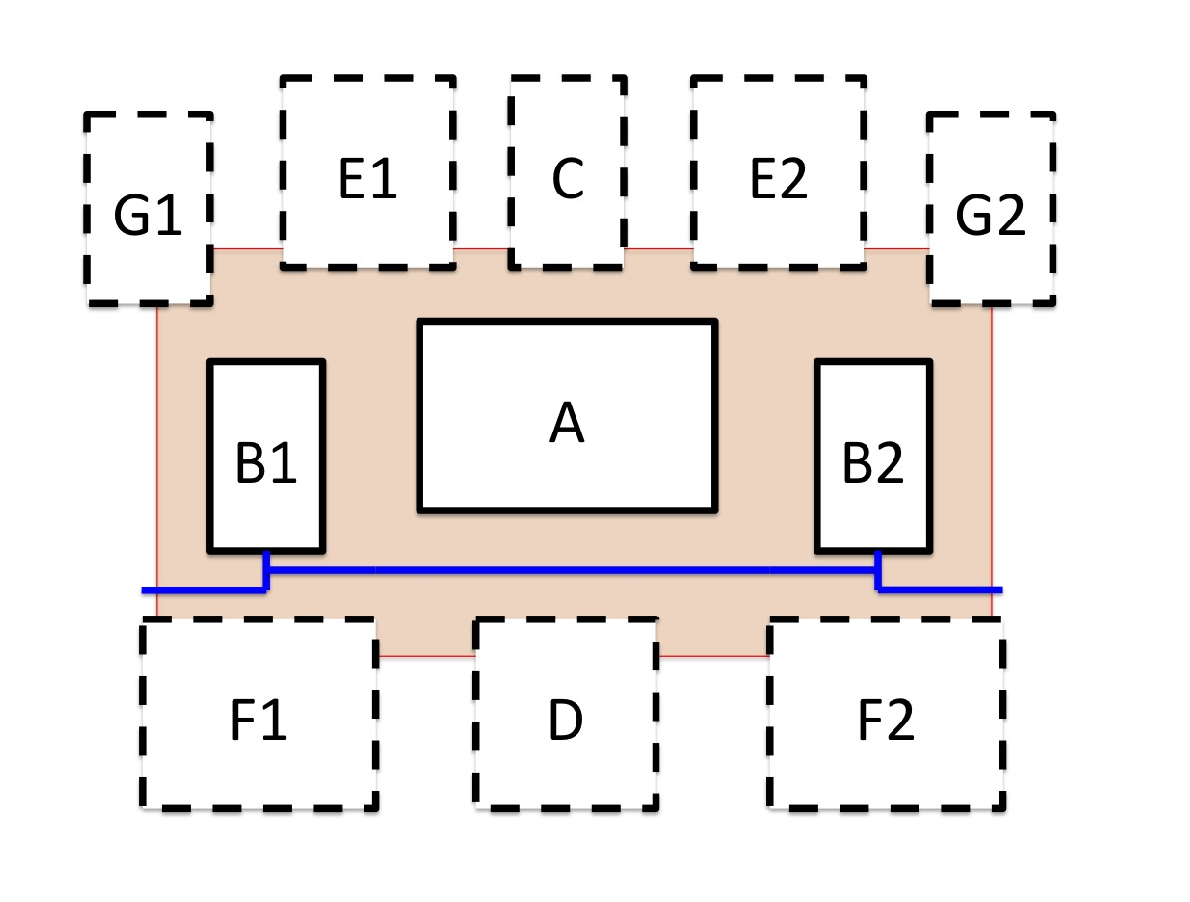
\includegraphics[width=4cm]{Fig/RoutingPreserv_b.eps}
    \caption{Non-preserved automatic routing}
    \label{fig:RoutingPreserv_B}
    \end{subfigure}
    %}
    \begin{subfigure}[t]{4cm}
    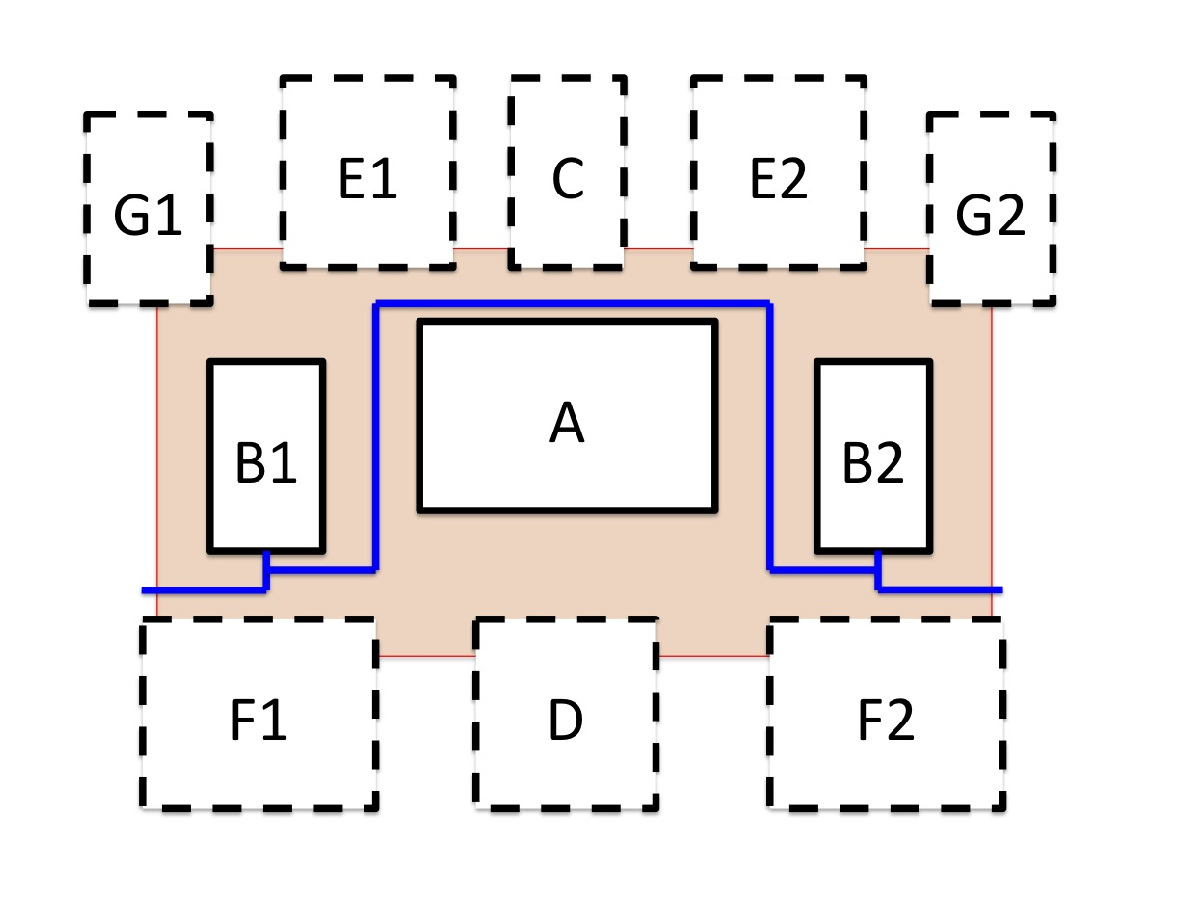
\includegraphics[width=4cm]{Fig/RoutingPreserv_c.eps}
    \caption{Preserved routing}
    \label{fig:RoutingPreserv_C}
    \end{subfigure}
    %}
    
    %\subfigure[Timing and simulation results]{
    %\label{fig:RoutingPreserv_d}
    %\epsfig{file=Fig/Prototyping_d.eps,width=4cm}
    %}
    \caption{Analog layout generation with different configuration. (a) Reference layout with complete placement and routing. (b) non-preserved automatic routing considering usual constraints only. (c) layout generation considering preserved routing characteristics. (d) simulation results in umc65nm technology.}
    \label{fig:RoutingPreserv}
  \end{figure}
%!TEX root = Thesis.tex

\chapter{Methodology and Table}\label{chap:Method}
      
        
  \begin{defi}
    {\bf way of def}: text here
  \end{defi}

  Example of equation in ~\ref{eq:devToCir}

  \begin{align}\label{eq:devToCir}
    \begin{array}[t]{rl}
      Variables: & \begin{array}[t]{rl}
                    T_{|V^D| \times S_{V^D}}  & = \{t_{i,j}| 1 \leq i \leq |V^D|,\; 1 \leq j \leq S_{V^D}\}   \\
                    V^C   &= \{v_j^C, 1\leq j \leq |V^C| \}   \\
                    v_j^C &= \{f_j^{(C_f)}(T_{|V^D| \times S_{V^D}})|1 \leq j \leq |V^C|\}  \\
                  \end{array} \\
       minimize & \| \sum{ v_j^C - f_j^{(C_f)}(T_{|V^D| \times S_{V^D}})}\|^2   \\
     subject\; to & C_f\in \left [{C_f}_{min}, {C_f}_{MAX} \right] 
    \end{array} 
  \end{align}


  \section{Experimental with Tables}\label{sec:PAGEExp}
    
    \newsavebox{\tablebox}
    \begin{table}[ht]
      \begin{center}
      {\small
        \caption{Device statistics of RFDA and OpAmp}\label{table:stat}
        \begin{lrbox}{\tablebox}
          \centering{
            \begin{tabular}{|c|c|c|c|c|c|}
              \hline
              &  \multicolumn{5}{c|}{Device Number} \\
              \cline{2-6}
              circuits &  MOS &   Capacitor & Resistor  &  Inductor & Total   \\
              \hline
              RFDA     &  12   &   30       &     0     &     30     &   72     \\
              \hline  
              Spec     &  $A_v(\frac{v}{v})$    & $P_{dc} (\mu W)$  & $P_{out}(mW)$  & $F_{cent}(GHz)$ & $BW(GHz)$   \\ 
              \cline{2-6}  
                       &  $ \geq5$ & $\leq 0.5$ & $\geq 2$& $\geq 5$ & $\geq 10$ \\
              \hline  
              Opamp   &  18   &    1       &     0     &      0     &   19     \\
              \hline  
              Spec     &  $A_v(\frac{v}{v})$    & $P_{dc} (\mu W)$  & $P_{out}(\mu W)$ & $BW(MHz)$   & Phase Margin  \\
              \cline{2-6}  
               &  $ \geq40$ & $\leq 100$ & $\geq 0.1 $& $\geq 60$ & $\geq 50$ \\
              \hline
            \end{tabular}
          }
          \end{lrbox}
        \scalebox{0.8}{\usebox{\tablebox}}
        }
      \end{center}
    \end{table}

    \definecolor{mygray}{gray}{.9}
    \begin{sidewaystable}
      \begin{center}
      \caption{The mapping results from circuit-level variables to performance metrics and the runtime from circuit-level to performance metrics for \cite{PerfMap_ISQED2011} and 3 genetic exploration styles.}    
      \label{table:PopulationResult}
      \begin{lrbox}{\tablebox}
        \centering{
        \begin{small}
        \begin{tabular}{|l|l|c|c|c|c|c|c|c|}
            \hline
            \rowcolor{mygray}
            RFDA        & Algorithm &Runtime(s) & Rumtime Improv.&    $A_v(\frac{v}{v})$    & $P_{dc} (\mu W)$  & $P_{out}(mW)$  & $F_{cent}(GHz)$           & $BW(GHz)$   \\ 
            \hline
            \cline{2-9}
                    & {\bf ITE}\cite{PerfMap_ISQED2011} &  38880 & - & 1.5- 8 & $\leq 0.85$ & $\leq 21.7$ &  $2.6802 \sim 27.299$     & $ 2.3485 \sim 51.587$ \\
            \cline{2-9}
                    & $\text G\text A_{64}$  & 4122  & 9.43x& 4 \~ 5.2143 & 0.368 - 0.997 & 20.9 - 21.2 &   11.0 - 13.56   & 18.92 - 24.10 \\
            \cline{2-9}
             umc65nm    & $\text P\text G\text A_{64}$  & 3416 & 11.38x&  4 - 5.2143 & 0.354 - 0.990  &  20.9 - 21.2 & 11.04 - 13.56& 19.07 - 24.10 \\
             \cline{2-9}
                    & $\text P\text G\text A_{256}$  & 8053 & 4.82x  & 4 - 5.2298 & 0.002 - 1.019 & 20.9 - 27.8 &  11.12 - 13.52   & 19.23 - 23.94 \\
            \hline
            \rowcolor{mygray}
            Opamp        & Algorithm &Runtime(s) & Runtime Improv. &   $A_v(\frac{v}{v})$    & $P_{dc} (\mu W)$  & $P_{out}(mW)$  & $PM$  & $BW(MHz)$   \\ 
            \hline
            \cline{2-9}
                    & {\bf ITE}\cite{PerfMap_ISQED2011} & 19432  & -  & 20 - 32.26 & $\leq 100$ & $\leq 0.65$  &  30\textdegree $\sim$  60\textdegree & $0.08 \sim 1.47$ \\
            \cline{2-9}
                    & $\text G\text A_{64}$ & 5958  & 3.26x  & 10 - 65.71 & 14 $\sim$ 100 & 0.1 $\sim$ 0.87 &   30\textdegree $\sim$ 72.85\textdegree   & $0.08 \sim 1.5$ \\
            \cline{2-9}
             umc65nm    & $\text P\text G\text A_{64}$  &1855 & 10.48x &  10 $\sim$ 91 & 28 $\sim$ 100  &  0.1 $\sim$ 1 & 30\textdegree $\sim$ 66\textdegree   & $0.1 \sim 1.5$  \\
             \cline{2-9}
                    & $\text P\text G\text A_{256}$  & 7992 & 2.43x  & 10 $\sim$ 91 & 14 $\sim$ 100 & 0.1 $\sim$ 1 &  30\textdegree $\sim$ 81\textdegree  & $0.1 \sim 1.5$ \\
            \hline
            \cline{2-9}
                    & {\bf ITE}\cite{PerfMap_ISQED2011} &  15285 & - & $20 \sim 46.77$ & $\leq 100$ &$\leq 0.65$  & 30\textdegree $\sim$ 60\textdegree &$0.08 \sim 1.47$  \\
            \cline{2-9}
                    & $\text G\text A_{64}$   & 4858  & 3.15x& 10 $\sim$ 145 & $14 \sim 100$ & 0.23 $\sim$ 1 &   38.57\textdegree $\sim$ 72.85\textdegree   &0.1 $\sim$ 1 \\
            \cline{2-9}
             umc90nm    & $\text P\text G\text A_{64}$ & 1813 & 8.43x &  10 $\sim$ 118 & 14 $\sim$ 85  &  0.1 $\sim$ 0.75 & 30\textdegree $\sim$ 81\textdegree & 0.1 $\sim$ 1.5  \\
             \cline{2-9}
                    & $\text P\text G\text A_{256}$  & 4037 & 3.79x & 10 - 400 & 1.28 - 30 & 0.25 - 0.89 &  30\textdegree $\sim$ 60\textdegree & 0.48 $\sim$ 1.5 \\
            \hline
            \cline{2-9}
                    & {\bf ITE}\cite{PerfMap_ISQED2011} & 19488 & -   & 20 $\sim$ 34.15 & $\leq 0.1$ & $\leq 0.91$  & 30\textdegree $\sim$ 60\textdegree  & 0.08 $\sim$ 1.47 \\
            \cline{2-9}
                    & $\text G\text A_{64}$  & 5918  & 3.29x &10 - 74.29 & 0.05 - 29.7 & 0.12 - 1.03 &  30\textdegree $\sim$ 60\textdegree   & 0.48 $\sim$ 1.5 \\
            \cline{2-9}
             tsmc90nm    & $\text P\text G\text A_{64}$ & 2805 & 6.94x &  10 - 74.29 & 0.14 - 28.68  &  0.18 - 1.03 & 30\textdegree $\sim$ 60\textdegree& 0.48 $\sim$ 1.5 \\
             \cline{2-9}
                    & $\text P\text G\text A_{256}$  & 7108 & 2.74x  & 10 - 74.29 & 0.13 - 29.69 & 0.17 - 0.96 &  30\textdegree $\sim$ 60\textdegree & 0.48 $\sim$ 1.5 \\
            \hline

        \end{tabular}
        \end{small}
        }
        \end{lrbox}
        \scalebox{0.8}{\usebox{\tablebox}}
      \end{center}
    \end{sidewaystable} 


    Table~\ref{table:stat} shows the statistics of the two circuits including the components of each and the typical performance specifications. Table~\ref{table:PopulationResult} show the table with sideway
      
    

    
%!TEX root = Thesis.tex

\chapter{Conclusions and Future Works}\label{chap:CFW}

  Conclusions

  \section{Conclusions}\label{sec:Conclusion}

    Showing the item and number funciton.
    \begin{itemize}
      \item item 1
      \item item 2
    \end{itemize}

    \begin{enumerate}
      \item first item
      \item second item
    \end{enumerate}




\backmatter
% !TEX root = Thesis.tex
% this file is encoded in utf-8
% v2.0 (Apr. 5, 2009)


%%%
\newpage
%\phantomsection % for hyperref to register this
%\addcontentsline{toc}{chapter}{\nameRef}
%\renewcommand{\bibname}{\protect\makebox[5cm][s]{\nameRef}}
%%  \makebox{} is fragile; need protect
\bibliographystyle{IEEEtran}  % �ϥ� IEEE Trans ���Z�榡
\bibliography{IEEEabrv,reference,reference_PAGE,reference_HCDR}


%%%
%\input{my_appendix.tex}

%%%
\newpage
\chapter*{\protect\makebox[\textwidth][c]{\nameVita}} % \makebox{} is fragile; need protect

\phantomsection % for hyperref to register this
\addcontentsline{toc}{chapter}{\nameVita}
%!TEX root = Thesis.tex

{\bf Po-Cheng Pan} received the B.S. degree in electronics engineering from National Chiao Tung University, Hsinchu, Taiwan, in 2007. 

From 2007, he we working his M.Sc. degree in electronics engineering. From 2009, he is currently pursuing the Ph.D. degree from the Institute of Electronics. He was a visiting scholar in Technical University of Munich in 2014 through DAAD program. His research interests includes analog circuit optimization, and analog circuit layout automaiton and migration. 

{\bf International Journal Papers}
\begin{enumerate}
  \item P.-C. Pan, C.-Y. Chin, H.-M. Chen, T.-C. Chen, C.-C. Lee and J.-C. Lin, ``A Fast Prototyping Framework for Analog Layout Migration with Planar Preservation,'' in \emph{IEEE Transactions on Computer-Aided Design of Integrated Circuits and Systems}, vol.pp, no.99, pp.1---1. 
\end{enumerate}
{\bf International Conference Papers}
\begin{enumerate}
  \item C.-Y. Chin, P.-C. Pan, H.-M. Cheng, T.-C. Chen, and J.-C. Lin, ``Efficient analog layout prototyping by layout reuse with routing preservation,'' in \emph{International Conference on Computer-Aided Design}, Nov. 2013, pp.40---47.
  \item P.-C. Pan, H.-M. Chen and C.-C. Lin, ``PAGE: Parallel agile genetic exploration towards utmost performance for analog circuit design,'' in \emph{Design, Automation and Testing in Europe Conference \& Exhibition}, Mar. 2013, pp.1849---1854.
  \item P.-C. Pan, H.-M. Chen, Y.-K. Cheng, J.~Liu, and W.-Y. Hu, ``Configurable analog routing methodology via technology and design constraint unification,'' in \emph{International Conference on Computer-Aided Design}, Nov. 2012, pp.620---626.
  \item Y.-P. Weng, H.-M. Chen, T.-C. Chen, P.-C. Pan, C.-H. Chen, and W.-Z. Chen, ``Fast analog layout prototyping for nanometer design migration,'' in \emph{International Conference on Computer-Aided Design}, Nov. 2011, pp. 517 -- 522.
  \item K.-H. Meng, P.-C. Pan, and H.-M. Chen, ``Integrated hierarchical synthesis of analog/rf circuits with accurate performance mapping,'' in \emph{International Symposium on Quality Electronic Design}, Mar. 2011, pp.1---8. 
  \item B.-Z. Chen, H.-M. Chen, L.-D. Huang and P.-C. Pan, ``A stochastic-based efficient critical area extractor on OpenAccess platform,'' in \emph{ACM Great Lake symposium on VLSI}, May 2009, pp.197---222.

\end{enumerate}



\end{document}
